\documentclass[letterpaper]{article}
\usepackage[margin=0.5in]{geometry}
\usepackage{tikz}
\usepackage[T1]{fontenc}
\usepackage[utf8]{inputenc}
\usepackage{lmodern}

\pagestyle{empty}
\setlength{\parindent}{0pt}

\begin{document}

\noindent
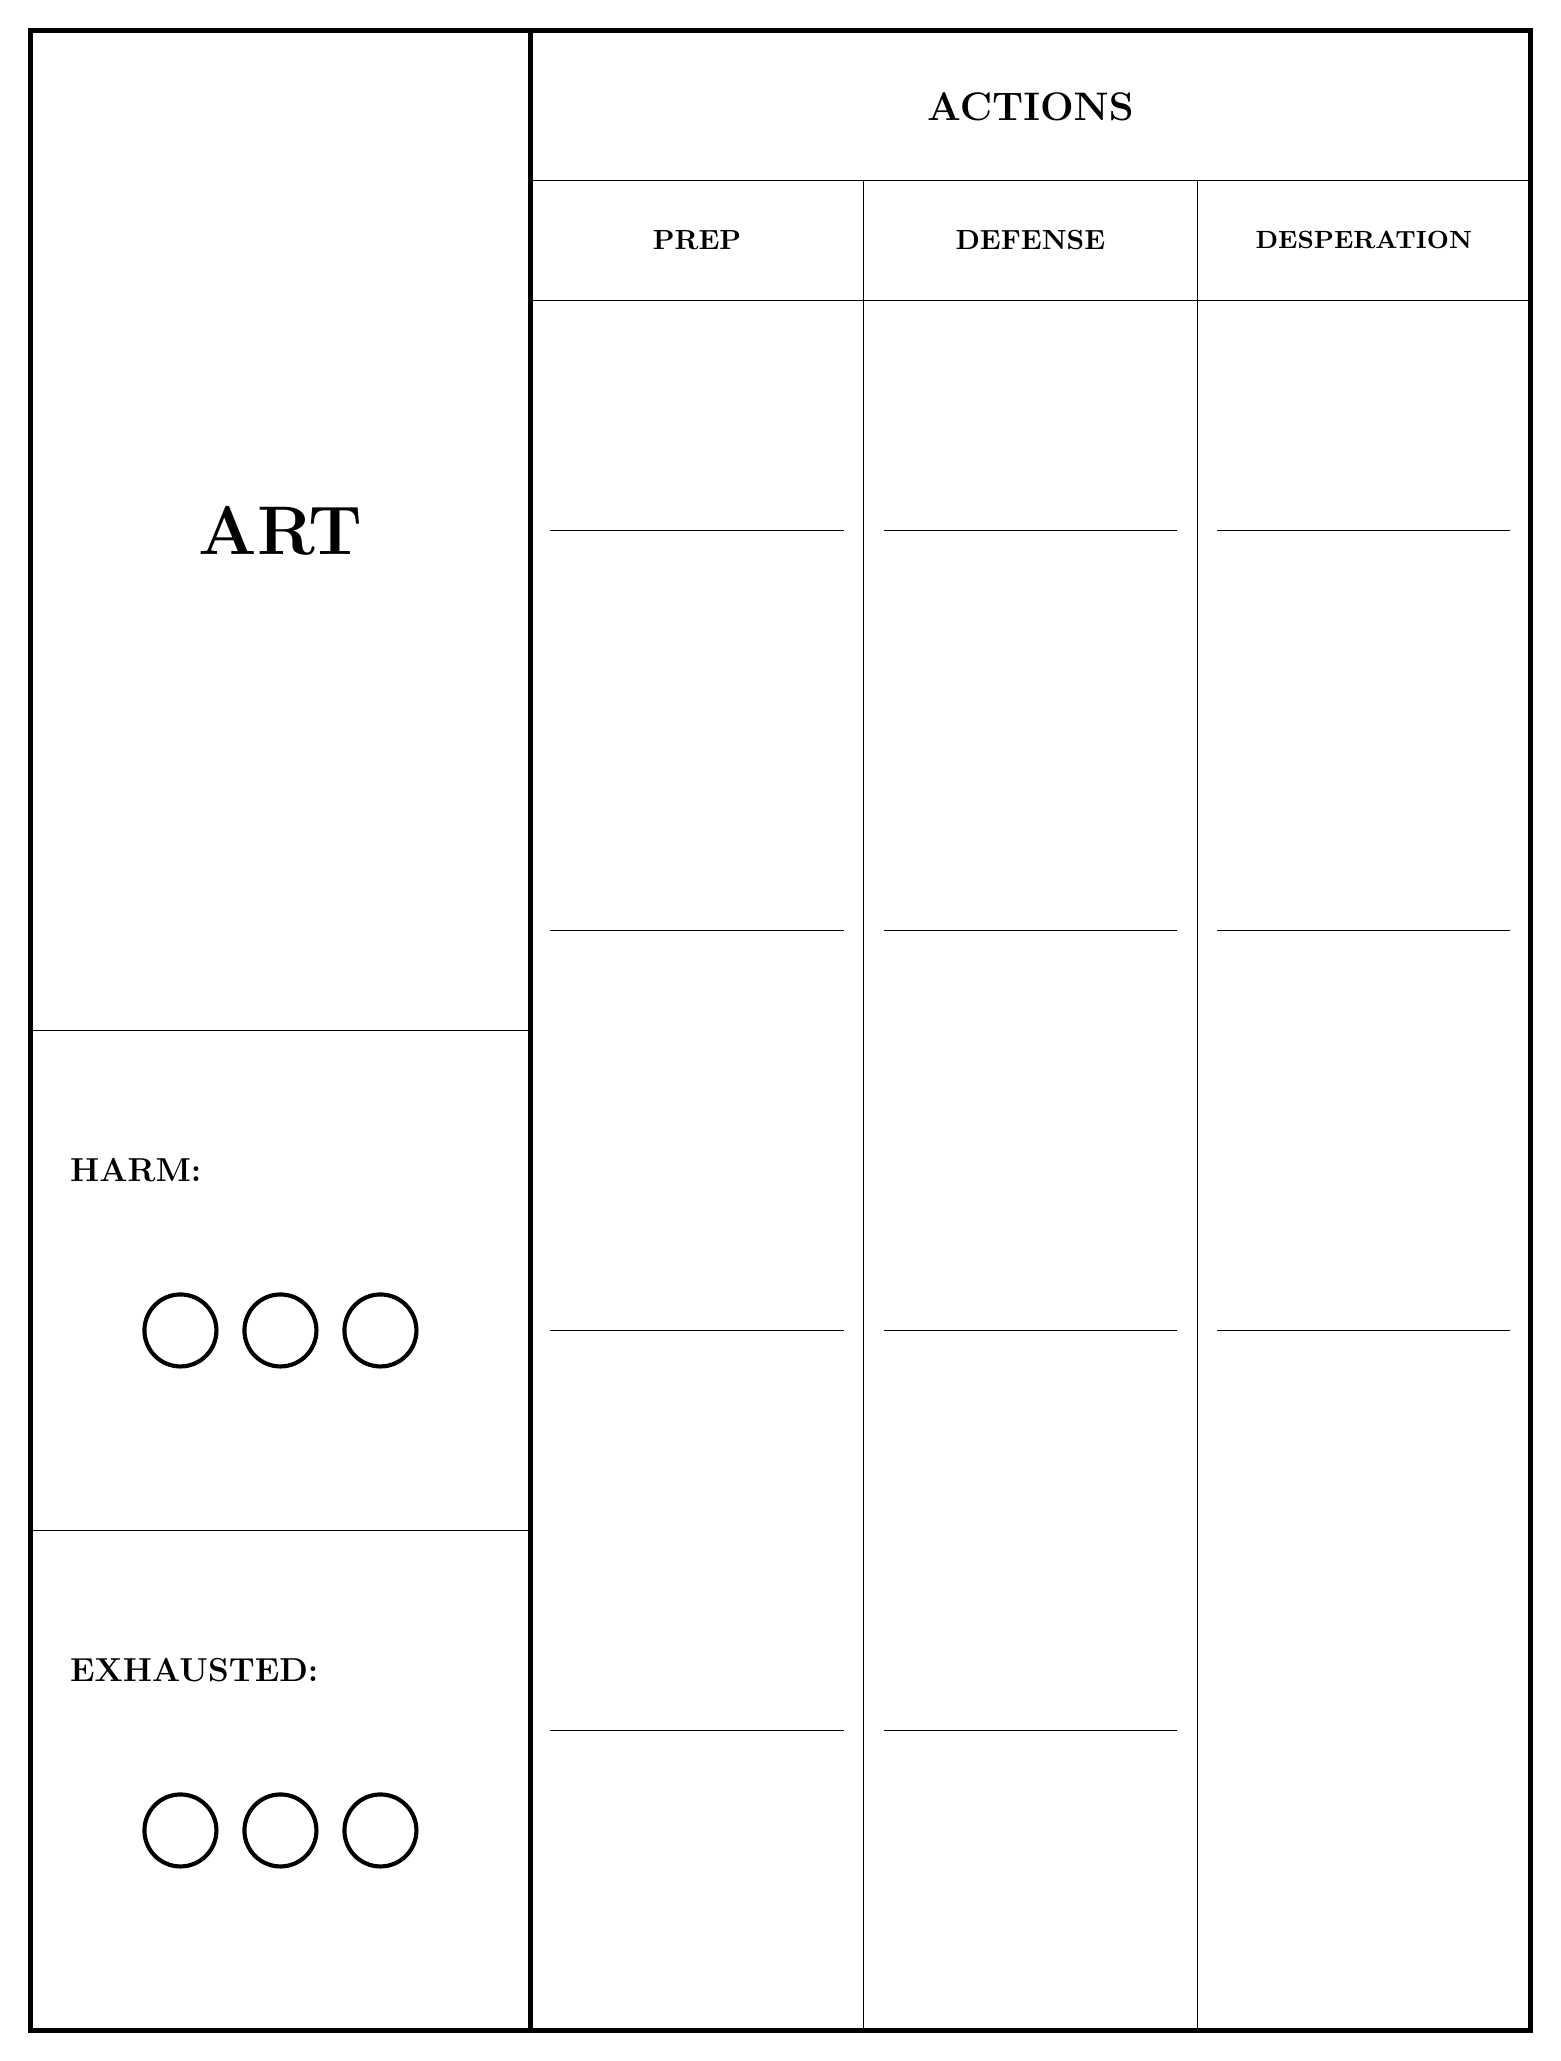
\begin{tikzpicture}[x=1in, y=-1in]

  %%-- OUTER BORDER --%%
  \draw[line width=2pt] (0,0) rectangle (7.5,10);

  %%-- LEFT COLUMN / RIGHT SECTION DIVIDER (x = 2.5") --%%
  \draw[line width=2pt] (2.5,0) -- (2.5,10);

  %%-- LEFT COLUMN HORIZONTAL DIVIDERS --%%
  \draw (0,5)   -- (2.5,5);    % bottom of ART box     (y = 5")
  \draw (0,7.5) -- (2.5,7.5);  % HARM / EXHAUSTED divider (y = 7.5")

  %%-- ART BOX LABEL (centered in 2.5" wide x 5" tall box) --%%
  \node[anchor=center] at (1.25,2.5) {%
    \fontsize{32}{38}\selectfont\textbf{ART}%
  };

  %%-- HARM ROW (y = 5" to 7.5") --%%
  \node[anchor=west] at (0.15,5.7) {\large\textbf{HARM:}};
  % Three circles centered horizontally in left column
  \foreach \cx in {0.75, 1.25, 1.75} {
    \draw[line width=1.5pt] (\cx,6.5) circle (0.18);
  }

  %%-- EXHAUSTED ROW (y = 7.5" to 10") --%%
  \node[anchor=west] at (0.15,8.2) {\large\textbf{EXHAUSTED:}};
  % Three circles centered horizontally in left column
  \foreach \cx in {0.75, 1.25, 1.75} {
    \draw[line width=1.5pt] (\cx,9.0) circle (0.18);
  }

  %%-- ACTIONS HEADER (spans full right section, y = 0" to 0.75") --%%
  \node[anchor=center] at (5.0,0.38) {\Large\textbf{ACTIONS}};
  \draw (2.5,0.75) -- (7.5,0.75);

  %%-- RIGHT SECTION: THREE EQUAL SUB-COLUMNS (5" / 3 = 1.667" each) --%%
  %% Sub-column dividers at x = 4.167" and x = 5.833"
  \draw (4.167,0.75) -- (4.167,10);
  \draw (5.833,0.75) -- (5.833,10);

  %%-- SUB-COLUMN HEADERS (y = 0.75" to 1.35") --%%
  \node[anchor=center] at (3.333,1.05) {\normalsize\textbf{PREP}};
  \node[anchor=center] at (5.000,1.05) {\normalsize\textbf{DEFENSE}};
  \node[anchor=center] at (6.667,1.05) {\small\textbf{DESPERATION}};
  \draw (2.5,1.35) -- (7.5,1.35);

  %%-- RULED LINES IN ACTION COLUMNS --%%
  %% 0.1" margin from sub-column borders on each side:
  %%   PREP column:        x = 2.6  to 4.067
  %%   DEFENSE column:     x = 4.267 to 5.733
  %%   DESPERATION column: x = 5.933 to 7.4
  %%
  %% Lines at y = 2.5, 4.5, 6.5 (shared by all three columns)
  %% 4th line at y = 8.5 for PREP and DEFENSE only (DESPERATION has 3 lines)
  \foreach \y in {2.5, 4.5, 6.5} {
    \draw (2.6,  \y) -- (4.067, \y);   %% PREP
    \draw (4.267,\y) -- (5.733, \y);   %% DEFENSE
    \draw (5.933,\y) -- (7.4,   \y);   %% DESPERATION
  }
  %% 4th line for PREP and DEFENSE
  \draw (2.6,  8.5) -- (4.067, 8.5);  %% PREP
  \draw (4.267,8.5) -- (5.733, 8.5);  %% DEFENSE

\end{tikzpicture}

\end{document}
